\subsection{Lebesgue's theorem}

THEOREM 6 (Lebesgue). --- Let F be a Banach space, \((\mathbf{f}_{n})\) a sequence of functions in \(L_{F}^{p}\) such that: \(1^{\circ}\) the sequence \((\mathbf{f}_{n}(x))\) converges almost everywhere to a limit \(\mathbf{f}(x) \in \mathrm{F}\) ; \(2^{\circ}\) there exists a numerical function \(g \geqslant 0\) such that \(\int^{*} g^{p} d|\mu| < +\infty\) and \(|\mathbf{f}_{n}(x)| \leqslant g(x)\) almost everywhere in X, for every integer n.~Then, the function f (defined almost everywhere) is p-th power integrable, and the sequence \((\mathbf{f}_{n})\) converges in mean of order p to f.

Consider the `double' sequence of numerical functions \(g_{mn} = |\mathbf{f}_m - \mathbf{f}_n|\) , which belong to \(\mathcal{L}^p\) (No.~5, Prop. 11); by hypothesis, \(\lim_{m\to \infty, n\to \infty}g_{mn}(x) = 0\) almost everywhere, and on the other hand \(|g_{mn}(x)|\leqslant 2g(x)\) almost everywhere; applying Cor. 3 of Th. 5 of No.~6 to this double sequence,

\[
\limsup _ {m \to \infty ,   n \to \infty} \mathrm{N} _ {p} (\mathbf {f} _ {m} - \mathbf {f} _ {n}) \leqslant \mathrm{N} _ {p} (0) = 0  ,
\]

and since \(\mathrm{N}_p(\mathbf{f}_m - \mathbf{f}_n) \geqslant 0\) this implies \(\lim_{m \to \infty, n \to \infty} \mathrm{N}_p(\mathbf{f}_m - \mathbf{f}_n) = 0\) ; in other words, the sequence \((\mathbf{f}_n)\) is a Cauchy sequence in \(\mathcal{L}_{\mathrm{F}}^p\) . The theorem therefore follows from Cor. 1 of Th. 3 of No.~4.

COROLLARY. --- Let A be a set of indices, filtered by a filter F having a countable base. If \((\mathbf{f}_{\alpha})_{\alpha \in \mathrm{A}}\) is a family of functions in \(L_{F}^{p}\) that, with respect to the filter \(\mathfrak{F}\) , converge pointwise almost everywhere to a function \(\mathbf{f}\) , and if, moreover, there exists a numerical function \(g \geqslant 0\) such that \(\int^{*} g^{p} d|\mu| < +\infty\) and \(|\mathbf{f}_{\alpha}(x)| \leqslant g(x)\) almost everywhere in \(X\) for each \(\alpha \in A\) , then the function \(\mathbf{f}\) is \(p\) -th power integrable and \(\mathbf{f}_{\alpha}\) tends in mean of order \(p\) to \(\mathbf{f}\) with respect to the filter \(\mathfrak{F}\) .

For, let \((\mathbf{A}_{n})\) be a decreasing countable base of F, and let \(\alpha_{n}\) be any element of \(A_{n}\) ; the sequence \((\mathbf{f}_{\alpha_{n}})\) converges pointwise to f almost everywhere in X, thus Th. 6 shows that f is p-th power integrable and that \(\lim_{n\to\infty}\mathrm{N}_{p}(\mathbf{f}-\mathbf{f}_{\alpha_{n}})=0\) . Since F is the intersection filter of the elementary filters associated with all such sequences \((\alpha_{n})\) (GT, I, §6, No.~8, Prop. 11), \(\lim_{\mathfrak{F}}\mathrm{N}_{p}(\mathbf{f}-\mathbf{f}_{\alpha})\) exists and is equal to the common limit 0 of all of the sequences \((\mathrm{N}_{p}(\mathbf{f}-\mathbf{f}_{\alpha_{n}}))\) .

\pandocbounded{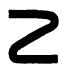
\includegraphics[keepaspectratio]{images/part001_1313f7e2.jpg}}

Remarks. --- 1) Th. 6 no longer holds if the hypothesis \(|\mathbf{f}_n| \leqslant g\) (with \(\mathrm{N}_p(g) < +\infty\) ) is replaced by the weaker hypothesis \(\sup_{n} \mathrm{N}_p(\mathbf{f}_n) < +\infty\) . Suppose, for example, that \(\mu\) is Lebesgue measure on \(\mathbf{R}\) ; define continuous functions \(f_n\) in the following manner: \(f_n(x) = 0\) for \(x \leqslant 0\) and for \(x \geqslant \frac{2}{n}\) , \(f_n(\frac{1}{n}) = n\) , \(f_n\) being linear on the intervals \([0, \frac{1}{n}]\) and \([\frac{1}{n}, \frac{2}{n}]\) . Then \(\lim_{n \to \infty} f_n(x) = 0\) for all \(x \in \mathbf{R}\) , but \(\mathrm{N}_1(f_n) = 1\) for every \(n\) (cf.~§5, Exer. 12).

\pandocbounded{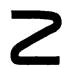
\includegraphics[keepaspectratio]{images/part001_8f7b1086.jpg}}

\begin{enumerate}
\def\labelenumi{\arabic{enumi})}
\setcounter{enumi}{1}
\tightlist
\item
  The Cor. of Th. 6 no longer holds if it is not assumed that the filter \(\mathfrak{F}\) has a countable base (cf.~§1, No.~3, Remark 1 following the Cor. of Th. 3).
\end{enumerate}

